% ------------------------------------------------------------------------------------
%                               CAPITOLO INTRODUTTIVO
% ------------------------------------------------------------------------------------
\chapter{Introduzione}

In questo corso sono trattati \textit{servizi di telecomunicazioni}.
Un servizio di telecomunicazioni permette a dispostivi diversi di
\textit{comunicare fra loro} ed è realizzato con un \textit{sistema di telecomunicazioni}.

\begin{definition}[SISTEMA DI TELECOMUNICAZIONI]
    Un \textit{sistema di telecomunicazioni} ha come obiettivo il \textit{trasporto di
    informazione} da una \textbf{sorgente} $A$ ad una \textbf{destinzazione} $B$. 
\end{definition}

\begin{figure}[!ht]
    \centering
    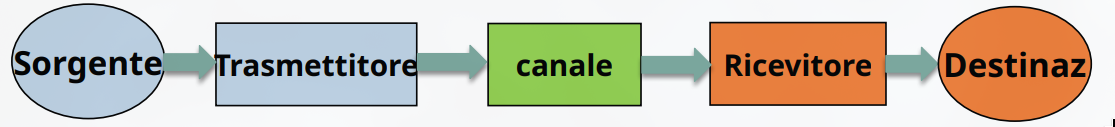
\includegraphics[width=0.8\textwidth]{images/01_01_SistemaTelecomunicazione.png}
    \caption{Sistema di Telecomunicazioni}
    \label{fig:01_01_SistemaTelecom}
\end{figure}

In particolare, come mostra la figura~\ref{fig:01_01_SistemaTelecom}, è composto dalle 
seguenti entità principali.
\begin{enumerate}
    \item \textbf{SORGENTE} : \textit{Genera informazione} sotto forma
        di una sequenza di simboli appartenenenti ad un \textit{alfabeto} $A$. 
        Spesso indicata con 'Tx'.
    \item \textbf{TRASMETTITORE}: \textit{Converte} la sequenza di
        simboli in una \textit{forma d'onda} (grandezza fisica, es tensione, onda
        elettromagnetica etc.) adatta ad essere trasmessa.
    \item \textbf{CANALE} : \textit{Mezzo fisico} (es cavo in ramo, fibra ottica, aria) 
        attraverso cui si propaga l'informazione.
    \item \textbf{RICEVITORE} : \textit{Elabora} l'informazione ricevuta.
        Spesso indicato con 'Rx'.
\end{enumerate}

% ----- RETI DI COMUNICAZIONE -----

\section{Reti di comunicazione}

I sistemi di telecomunicazioni sono \textit{interconnessi} a formare 
\textbf{reti di comunicazione}, come mostra la figura~\ref{fig:01_02_ReteTelecom}:

\newpage

\begin{figure}[!ht]
    \centering
    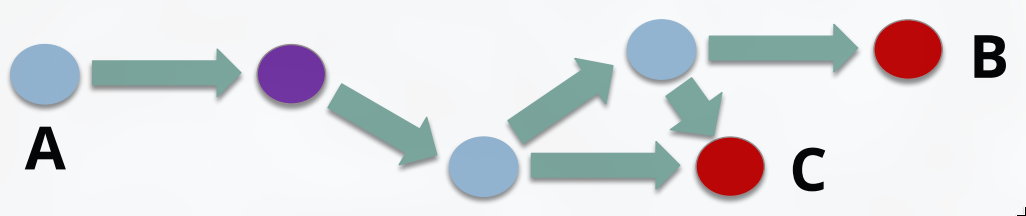
\includegraphics[width=0.8\textwidth]{images/01_02_RetiTelecom.png}
    \caption{Rete di Telecomunicazioni}
    \label{fig:01_02_ReteTelecom}
\end{figure}

\begin{remark}[RUOLI DINAMICI]
    I \textbf{ruoli non sono fissi}: ciascun nodo della rete può 
    essere sia trasmettitore che ricevitore.
\end{remark}

\subsection{Tipologie di comunicazione}

Possiamo classificare la comunicazione in base alle seguenti categorie:
\begin{itemize}
    \item \textbf{UNICAST} : Da \textit{punto a punto}.
    \item \textbf{MULTICAST} : Da un nodo ad \textit{altri punti}.
    \item \textbf{BROADCAST} : Da un nodo \textit{a tutti gli altri}.
\end{itemize}

\subsection{Direzione della comunicazione}

Un servizio può essere classificato come:
\begin{itemize}
    \item \textbf{UNIDIREZIONALE} (es. televisione)
    \item \textbf{BIDIREZIONALE}
        \begin{itemize}
            \item \textit{ASIMMETRICO} (es. web browsing)
            \item \textit{SIMMETRICO} (es. telefono)
        \end{itemize}
\end{itemize}

In particolare, i sistemi biderezionali sono a loro volta classificati anche in:
\begin{itemize}
    \item \textbf{HALF-DUPLEX} : la trasmissione può avvenire in entrambe le direzioni, ma
        \textit{non contemporaneamente}.
    \item \textbf{FULL-DUPLEX} : la trasmissione può avvenire nelle 
        due direzioni \textit{contemporaneamente}.
\end{itemize}

% ----- RUMORE E INTERFERENZE -----

\section{Rumore e Interferenze}

Ciascun entità del sistema di telecomunicazione è una possibile \textbf{fonte di rumore},
in particolare lo è il \textbf{canale}, a causa di \textit{rumore termico} e altre
\textit{distorsioni fisiche}.

\begin{definition}[RUMORE]
    Il rumore (o \textit{interferenza}) è una \textbf{fonte di errori}
    nella \textit{sequenza di simboli}.
\end{definition}

In altre parole, il rumore introduce \textbf{errori nei simboli trasmessi}.

Alla luce di ciò, si definiscono (per esempio):
\begin{itemize}
    \item \textbf{SNR} (\textit{Signal to Noise Ratio}) : Rapporto segnale/rumore, che quantifica
        la qualità dell'informazione ricevuta rispetto all'originale.
    \item \textbf{BER} (\textit{Bit Error Rate}) : Nelle trasmissioni \textit{digitali} quantifica
        la probabilità di \textit{errore su un bit} ($P_{\text{bit}}\coloneqq P[\hat{b}_k \ne b_k]$).
\end{itemize}
